\section{Results}

\subsection{gem5 CPU model accuracy}

After modelling different configurations for gem5, accuracy as depicted in \autoref{tbl:gem5runtimeaccuracy}
was achieved. Each test was run with the command written out in \autoref{lst:gem5commandline}, with \texttt{CPU}
changed with  \texttt{exynos\_4412p}, \texttt{arm\_detailed} and \texttt{timing}.

\begin{lstlisting}[language=sh,label={lst:gem5commandline},caption={gem5 Command Line}]
$ build/ARM/gem5.opt --remote-gdb-port=0 -d m5out-time/sha2-sha2
    configs/example/se.py -c bin/sha2/sha2 --cpu-type=CPU
    --mem-type=LPDDR2_S4_800_x32 --sys-clock=440MHz
    --cpu-clock=1700MHz --num-l3caches=0 --caches --l2cache
    --l2_assoc=16 --l2_size=1MB --l1d_size=32kB
    --mem-size=2048MB --l1d_assoc=4 --l1i_assoc=4
\end{lstlisting}


% Move table to result chapter
\begin{table}
\centering
\begin{tabular}{|l|c|c|c|c|}
\hline
 & add-add & pi-pi & sha2-sha2 & trend-trend \\
\hline
Real hardware & 0.017600  & 0.013500 & 0.022600 & 0.014600 \\
gem5 modified O3    & 0.017541 & 0.013790 & 0.022819 & 0.011898 \\
gem5 original O3    & 0.008777 & 0.006708 & 0.010368 & 0.004344 \\
gem5 timing simple  & 0.035039 & 0.019564 & 0.040659 & 0.020503 \\
\hline
\end{tabular}
\caption{gem5 runtime accuracy (O3 with classic memory system)}
\label{tbl:gem5runtimeaccuracy}
\end{table}




\subsection{GA optimization}
As PET has been optimized by a genetic inspired algorithm, it is likly to perform very well on the data sets it
has been optimized for. When such training is done, a controll test is needed in order to verify that the result
is good for the general problem solved, not only the specific instances used for training.

\subsection{Training}

The training sets:
\begin{figure}
\centering
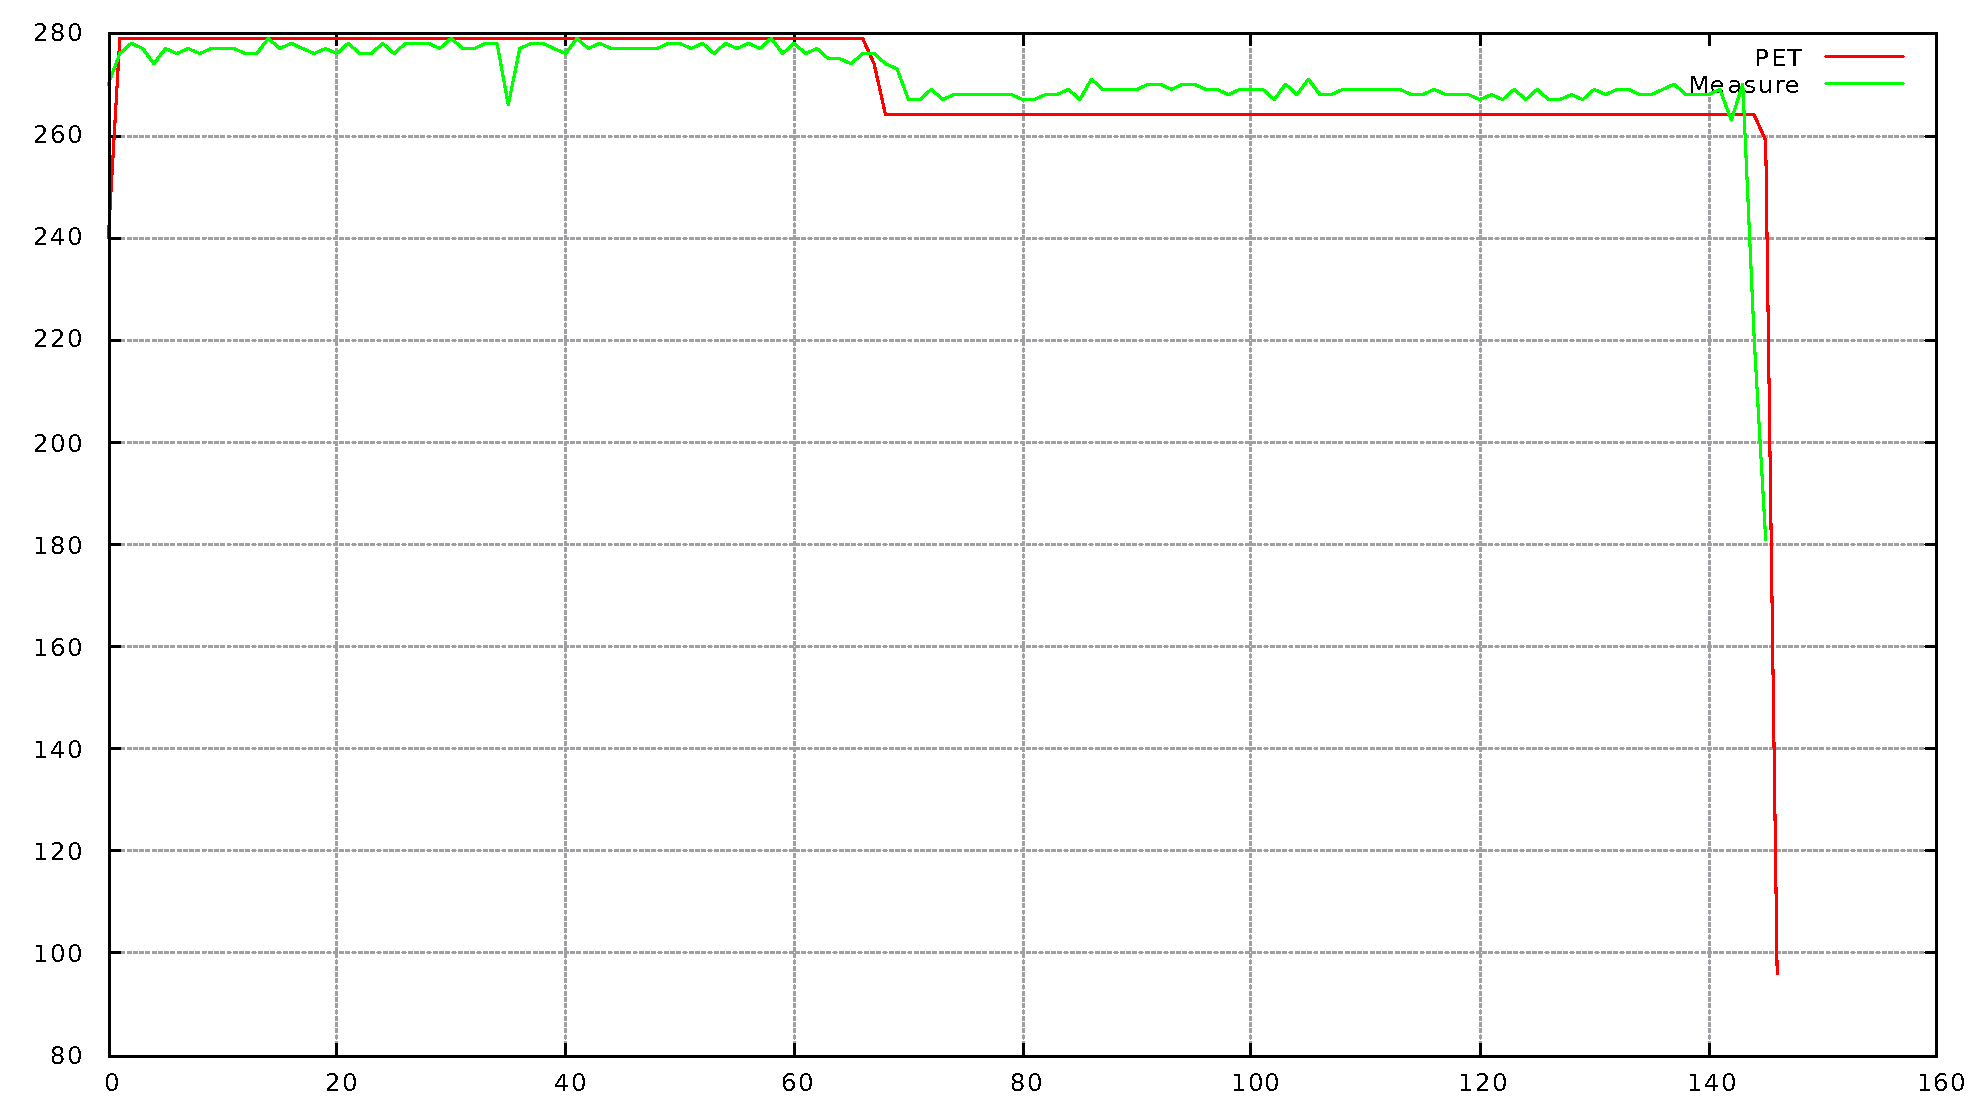
\includegraphics[width=\textwidth]{figs/trend-training.pdf}
\caption{Overlay of PET training results (red) and training data (green)}
\label{fig:trend-training}
\end{figure}

